

\def\full{0} %% set to 0 for springer proceedings


\ifnum\full=1
\documentclass[11pt]{llncs}
\addtolength{\parskip}{1pt}
\else
\documentclass[10pt, runningheads]{llncs}
\usepackage{times}
\fi




\usepackage{makeidx}
\usepackage[dvips]{graphicx}
\usepackage{graphicx}

\usepackage{comment}

\usepackage{listings}
\usepackage[mathscr]{eucal}
\usepackage{bm}
\usepackage{array}
\usepackage{url}
\usepackage{calc}
\usepackage{float}
\usepackage{latexsym}
\usepackage{rotating}
\DeclareGraphicsExtensions{.eps,.jpg,.png,.pdf}
\usepackage[usenames, dvipsnames]{xcolor}
\usepackage[sort,nocompress]{cite}
\usepackage{colortbl}
\usepackage{multirow}
\usepackage{lscape}
\usepackage{amsmath}
\let\proof\relax
\let\endproof\relax
\usepackage{amsthm,amsfonts,amssymb}
\usepackage{hyperref}
\usepackage{pdflscape}


%\usepackage{natbib}

\def\rmdefault{ptm}



\usepackage{setspace}
\usepackage{color}
\ifnum\full=1
\usepackage[margin=0.9in]{geometry}
\usepackage{fullpage}

\setlength{\parskip}{0cm}

%\setstretch{1.03}
%\addtolength{\parskip}{1pt}
\setcounter{page}{0}
\renewcommand{\tabcolsep}{5pt}
\else
\renewcommand{\tabcolsep}{0pt}
\fi

\renewcommand{\arraystretch}{1.2}

\hyphenpenalty=5000
\tolerance=1000




%\ifnum\full=1
%\usepackage{natbib}
%\bibliographystyle{alpha}
%\setlength{\bibsep}{0pt}
%\renewcommand{\bibsection}{\section*{References}\small}
%\else
%\usepackage[numbers]{natbib}
%\bibliographystyle{splncs04}
%\fi



\DeclareMathOperator{\Exp}{E}
\DeclareMathOperator{\Var}{Var}
\DeclareMathOperator{\poly}{poly}
\DeclareMathOperator{\Supp}{Supp}

\usepackage{enumitem}


\usepackage{tikz}
\usetikzlibrary{arrows,shapes}
\usetikzlibrary{plotmarks}


%notes

%\definecolor{myorange}{rgb}{0.99,0.6,0.25}
%\newcommand{\pmnote}[1]{\colorbox{myorange}{\parbox{0.9\linewidth}{[{\footnotesize {\bf PM:} { {#1}}}]}}}


\definecolor{mycolor}{rgb}{0.75,0.95,0.05}
\newcommand{\pmnote}[1]{\colorbox{mycolor}{\parbox{0.9\linewidth}{[{\footnotesize {\bf PM:} { {#1}}}]}}}

\definecolor{color2}{rgb}{0.95,0.9,0.2}
\newcommand{\lbnote}[1]{\colorbox{color2}{\parbox{0.9\linewidth}{[{\footnotesize {\bf LB:} { {#1}}}]}}}


%% Sets

\newcommand{\Z}{\mathbb{Z}}
\newcommand{\N}{\mathbb{N}}
\newcommand{\R}{\mathbb{R}}
\newcommand{\F}{\mathbb{F}}
\newcommand{\Znm}{\mathbb{Z}_q^{n \times m}}

%matrices
\newcommand{\matzero}{\mathbf{0}}
\newcommand{\matA}{\mathbf{A}}
\newcommand{\matB}{\mathbf{B}}
\newcommand{\matC}{\mathbf{C}}
\newcommand{\matE}{\mathbf{E}}
\newcommand{\matF}{\mathbf{F}}
\newcommand{\matG}{\mathbf{G}}
\newcommand{\matI}{\mathbf{I}}
\newcommand{\matM}{\mathbf{M}}
\newcommand{\matP}{\mathbf{P}}
\newcommand{\matR}{\mathbf{R}}
\newcommand{\matS}{\mathbf{S}}
\newcommand{\matT}{\mathbf{T}}
\newcommand{\matU}{\mathbf{U}}
\newcommand{\matV}{\mathbf{V}}
\newcommand{\matW}{\mathbf{W}}
\newcommand{\matX}{\mathbf{X}}
\newcommand{\matY}{\mathbf{Y}}
\newcommand{\matZ}{\mathbf{Z}}


%vectors
\newcommand{\veca}{\mathbf{a}}
\newcommand{\vecb}{\mathbf{b}}
\newcommand{\vecc}{\mathbf{c}}
\newcommand{\vecd}{\mathbf{d}}
\newcommand{\vece}{\mathbf{e}}
\newcommand{\veci}{\mathbf{i}}
\newcommand{\vecj}{\mathbf{j}}
\newcommand{\veck}{\mathbf{k}}
\newcommand{\vecl}{\mathbf{l}}
\newcommand{\vecm}{\mathbf{m}}
\newcommand{\vecp}{\mathbf{p}}
\newcommand{\vecr}{\mathbf{r}}
\newcommand{\vecs}{\mathbf{s}}
\newcommand{\vecv}{\mathbf{v}}
\newcommand{\vecw}{\mathbf{w}}
\newcommand{\vecu}{\mathbf{u}}
\newcommand{\vecx}{\mathbf{x}}
\newcommand{\vecy}{\mathbf{y}}
\newcommand{\vecz}{\mathbf{z}}





%FiLIP notations

\newcommand{\FLIP}{\textsf{FLIP}}
\newcommand{\IFPl}{\text{Improved Filter Permutator} }
\newcommand{\IFPs}{\text{IFP} }

\newcommand{\FiLIP}{\textsf{FiLIP}}
\newcommand{\FiLIPDSM}{\mathsf{FiLIP}_{\mathsf{DSM}}}
\newcommand{\FiLIPXMAJ}{\mathsf{FiLIP}_{\mathsf{XMAJ}}}

%Boolean functions

\newcommand{\Bfn}[1]{\mathcal{B}_{#1}}
\newcommand{\BN}{\mathcal{B}_n}
\newcommand{\Bn}[1]{\mathcal{B}_{#1}}
\newcommand{\Bnstar}[1]{\mathcal{B}_{#1}^*}

\newcommand{\Bvad}[3]{\mathcal{B}({#1},{#2},{#3})}


\newcommand{\AI}{\mathsf{AI}}
\newcommand{\AIk}[1]{\mathsf{AI}_{#1}}
\newcommand{\AN}{\mathsf{AN}}
%\newcommand{\difAN}[1]{\Delta_{\mathsf{AN}}(#1)}
%\newcommand{\DAN}{\mathsf{d}\mathsf{AN}}
%\newcommand{\Sd}{\mathsf{S}_\mathsf{d}}
\newcommand{\SD}{\mathsf{SD}}
\newcommand{\FAI}{\mathsf{FAI}}
\newcommand{\NL}{\mathsf{NL}}
\newcommand{\NLk}[1]{\mathsf{NL}_{#1}}
%\newcommand{\NLd}{\mathsf{NL_d}}
\newcommand{\res}{\mathsf{res}}
\newcommand{\bal}{\mathsf{bal}}
\newcommand{\gnlk}{\mathsf{GWNL}}


\newcommand{\DS}[1]{\mathsf{DS}(#1)}
\newcommand{\DSR}[2]{\mathsf{DS}^{#2}(#1)}
%\newcommand{\matAI}[3]{\mathbf{A}_{#2,#3}(#1)}

\newcommand{\WPB}[1]{\mathcal{WPB}_{#1}}
\newcommand{\WAPB}[1]{\mathcal{WAPB}_{#1}}
\newcommand{\SWAPB}[1]{\mathcal{SWAPB}_{#1}}
\newcommand{\SYM}[1]{\mathcal{SYM}_{#1}}
%for affine weightwise: degree and number of variables
\newcommand{\WD}[2]{\mathcal{WD}^{#1}_{#2}}
\newcommand{\Ekn}[2]{\mathsf{E}_{#1,#2}}
\newcommand{\Code}[2]{\mathsf{P}_{#1,#2}}
\newcommand{\mdist}[2]{\mathsf{d}_{#1,#2}}


\newcommand{\mnlk}[2]{\mu_{#1,#2}}
\newcommand{\Mnlk}[2]{\mathsf{M}_{#1,#2}}
\newcommand{\mnl}[1]{\mu_{#1}}
\newcommand{\Mnl}[1]{\mathsf{M}_{#1}}

\newcommand{\DistWkn}[2]{\mathfrak{W}_{#1,#2}}
\newcommand{\DistWn}[1]{\mathfrak{W}_{#1}}
\newcommand{\Dkn}[2]{\mathfrak{D}_{#1,#2}}
\newcommand{\Dn}[1]{\mathfrak{D}_{#1}}

\newcommand{\kraw}[3]{\mathsf{K}_{#1}(#2,#3)}
\newcommand{\phikn}[2]{\varphi_{#1,#2}}

\newcommand{\const}[2]{g_{#1,#2}}
\newcommand{\setn}[1]{S_{#1}}
\newcommand{\symsetsmall}[1]{A_{#1}}
\newcommand{\symset}[2]{B_{#1,#2}}


%usual notations
\newcommand{\supp}{\mathsf{supp}}
\newcommand{\suppk}[1]{\mathsf{supp}_{#1}}
\newcommand{\w}{\mathsf{w_H}}
\newcommand{\hd}{\mathsf{d_H}}
\newcommand{\degg}{\mathsf{deg}}
\newcommand{\Span}{\mathsf{Span}}
\newcommand{\rank}{\mathsf{rank}}
%Walsh transform
\newcommand{\wt}[1]{W_{#1}} 
\newcommand{\Wsupp}[1]{\mathsf{Wsupp}_{#1}} 
%restricted Walsh transform W_k,a (f)
\newcommand{\wtk}[2]{\mathcal{W}_{#1,#2}} 

%S-equivalent classes
\newcommand{\sclass}[1]{\mathcal{S}(#1)}


\newcommand{\set}[1]{\left\{#1\right\}}
\newcommand{\mAN}[1]{\mathsf{d}_{#1}}


%gates
\newcommand{\AND}{\textsf{AND}}
\newcommand{\XOR}{\textsf{XOR}}
\newcommand{\MUX}{\textsf{MUX}}


%families of functions
\newcommand{\MAJ}{\textsf{MAJ}}
\newcommand{\DSM}{\textsf{DSM}}
\newcommand{\XORTHR}{\textsf{XOR-THR}}
\newcommand{\XORMAJ}{\textsf{XOR-MAJ}}

\newcommand{\xorlk}[2]{{\mathsf{XOR}}_{#1}  \mathsf{M}_{#2}} 
\newcommand{\xormaj}[2]{{\mathsf{XOR}}_{#1}  \mathsf{MAJ}_{#2}} 
%\newcommand{\xorthr}[3]{{\mathsf{XOR}}_{#1}  \mathsf{T}_{{#2},{#3}}} 
\newcommand{\xorthr}[3]{{\mathsf{XOR}}_{#1}+\mathsf{T}_{{#2},{#3}}}
\newcommand{\tri}[1]{{T}_{#1}}
\newcommand{\thr}[2]{\mathsf{T}_{{#1},{#2}}}
\newcommand{\xor}[1]{\mathsf{XOR}_{#1}}
\newcommand{\maj}[1]{\mathsf{MAJ}_{#1}}


\newcommand{\nbf}[1]{\mathsf{C}_{#1}}
\newcommand{\nbfodd}[2]{\mathsf{A}_{#1,#2}}
\newcommand{\nbfeven}[2]{\mathsf{B}_{#1,#2}}

%direct sum vector and simplified value vector
\newcommand{\dsv}[1]{\mathbf{m}_{#1}}
\newcommand{\svv}[1]{\mathbf{s}_{#1}}



\newtheorem{Prop}{Property}
\newtheorem{Cons}{Construction}


% For algorithms
\usepackage{algorithm,algpseudocode}

\renewcommand{\algorithmicrequire}{\textbf{Input:}}
\renewcommand{\algorithmicensure}{\textbf{Output:}}
% \renewcommand{\ALG@name}{Construction}
\newenvironment{constr}[1][htb]{%
\floatname{algorithm}{Construction}% Update algorithm name
   \begin{algorithm}[#1]%
  }{\end{algorithm}}
 
\algnewcommand\algorithmicparfor{\textbf{par-for}}
\algdef{S}[FOR]{ParFor}[1]{\algorithmicparfor\ #1\ \algorithmicdo}
 
%latin

\newcommand{\ie}{\textit{i.e.} }
\newcommand{\eg}{\textit{e.g.} }
\newcommand{\ea}{\textit{et al.} }




\usepackage{float}
\usepackage{placeins}
\usepackage{caption}
\usepackage{subcaption}
\usepackage{booktabs}  % For better table formatting
\usepackage{array}     % Allows better column width control
\usepackage{graphicx} 

\usepackage{xr-hyper}
\usepackage{hyperref}
\externaldocument{restrictedAI}

\begin{document}
\appendix
\setcounter{algorithm}{1}
\section{Proofs}\label{sec:proofs}
In this section, we provide the proof of the propositions given in the article. 
For each proposition, we re-state the statement and we provide the corresponding proof.
\subsection{Proof of Proposition~\ref{prop:constantFs}.}
\begin{description}
    \item[Statement:] A Boolean function $f$ has an $\AI_S$ of $0$ if and only if the restriction $f_S$ on $S$ is constant.
\end{description}

\begin{proof}
	First, we show the reverse implication.
	We suppose that $f\in \BN$ is constant on $S$, either $f(x) = 0$ for all $x\in S$, or $f(x) = 1$ for all $x\in S$.
	If $f$ is not null everywhere but $f(x) = 0\ \forall x \in  S$, then the constant function $g(x) = 1$ is not zero on all $S$, and is it such that $g(x)f(x) = 0$ for all $x\in S$. 
	Similarly, if for all $x\in S$ $f(x) = 1$, the same argument can be used for the function $f+ 1$ on $S$.
	
	Then, we show the direct implication.
	We suppose that a function $g\in \BN$ is a non-zero-annihilator of $f$ restricted to $S$ of degree $0$. Then,
	$g \neq 0$ and $\deg(g) = 0 \Rightarrow g = 1$, therefore since $g$ annihilates $f$ in $S$,  $g(x) f(x) = 0$ for all $x \in S$, resulting in $f(x)g(x) = f(x) = 0$.
	Similarly, if $g$ annihilates $f+ 1$ on $S$ instead of $f$, we have that $g(x)(f(x) + 1) = 0$ implying that $f+ 1 = 0 \Rightarrow f(x) = 1$ for all $x\in S$. 
\end{proof}

\subsection{Proof of Proposition~\ref{prop:compareranks}.}
\begin{description}
    \item[Statement:] Let $Z = \supp\left(f^{(o)}\right) \cap S$.
If $\text{rank}\left(G^{f_{Z}^{(o)},S}_{r,n}\right) < \text{rank}(G^{S}_{r,n})$, then $f^{(o)}$ admits a non-zero-annihilator restricted to $S$ of degree at most $r$.
\end{description}

\begin{proof}
	Let $D_r^n = \sum_{i=0}^r \binom{n}{i}$. Since $D_r^n = \text{rank}(G^{f^{(o)}_S,S}_{r,n}) + |\text{Ker}(G^{f^{(o)}_S,S}_{r,n})| =  \text{rank}(G^{S}_{r,n}) + |\text{Ker}(G^{S}_{r,n})|$, we have that
	$\text{rank}(G^{f_S^{(o)},S}_{r,n}) < \text{rank}(G^{S}_{r,n}) \iff |\text{Ker}(G^{f_S^{(o)},S}_{r,n})| > |\text{Ker}(G^{S}_{r,n})|$. 
	Therefore $\exists v\in \text{Ker}(G^{f_S^{(o)},S}_{r,n}) \mbox{ such that }v\not\in \text{Ker}(G^{S}_{r,n})$. 
	Hence, it exists a Boolean function $g$ of degree $r$, whose truth table is given by $v \cdot G_{r,n}$, which is such that $v \cdot G_{r,n}\neq 0$ and $v \cdot G_{r,n}^{S}\neq 0$, but $(g \cdot f_S^{(o)})_S = v \cdot G_{r,n}^{f_S^{(o)},S} = 0$.
	Since $\text{rank}\left(G_{r,n}^{f_S^{(o)}, S}\right) = \text{rank}\left(G_{r,n}^{f^{(o)}, S}\right)$, $\text{rank}(G^{f^{(o)},S}_{r,n}) < \text{rank}(G^{S}_{r,n}) \Rightarrow \text{rank}(G^{f_Z^{(o)},S}_{r,n}) < \text{rank}(G^{S}_{r,n})$ and hence the condition $\text{rank}(G^{f_Z^{(o)},S}_{r,n}) < \text{rank}(G^{S}_{r,n})$ is enough to justify the existence of such $v$ giving the non-zero-annihilator $g$ of $f^{o}$ restricted to $S$.
\end{proof}

\subsection{Proof of Proposition~\ref{prop:swappingElementOfZToReduceKer}}
\begin{description}
    \item[Statement:] Let $k < \min\{(|Z|, |E_{D_n^n}|\}$ and let $V_k$ constructed following Definition~\ref{def:inductiveConstructionOfV}. 
    Suppose $\text{ker}(V_k) = \langle \hat{g}_k \rangle=\langle (\epsilon_1, \epsilon_2, \dots, \epsilon_k) \rangle $ and let $g_k\in \Bn{n}$ be the Boolean function having $\hat{g}_k$ as ANF. 
    Furthermore, assume there exists a $z_{k+j}$, for $j\geq 1$ such that $g_k(z_{k+j}) = 1$. Then, the matrix $V^{'}_{k+1}$ constructed as:
    \begin{align*}
        V^{'}_{k+1} = 
        \begin{pmatrix}
        \multicolumn{4}{c}{\multirow{4}{*}{$V_{k}$}} & z_{k+j}^{\alpha_{1}}\\
        & & & & z_{k+j}^{\alpha_{2}}\\
        & & & & \vdots\\
        & & & & z_{k+j}^{\alpha_{k}}\\
        z_{1}^{\alpha_{k+1}} & z_{2}^{\alpha_{k+1}}& \cdots & z_{k}^{\alpha_{k+1}} & z_{k+j}^{\alpha_{k+1}}
    \end{pmatrix}
    \end{align*}
    is such that $(\epsilon_1, \epsilon_2, \dots, \epsilon_k, 0) \not\in \text{ker}(V^{'}_{k+1})$. 
\end{description}

\begin{proof}
	
	    Suppose \( \text{ker}(V_k) = \langle \hat{g}_k \rangle = \langle (\epsilon_1, \epsilon_2, \dots, \epsilon_k) \rangle \), and that there exists \( j \geq 1 \) such that \( g_k(z_{k+j}) = 1 \), but it is also such that \( (\epsilon_1, \epsilon_2, \dots, \epsilon_k, 0) \in \text{ker}(V'_{k+1}) \).

  
If \( (\epsilon_1, \epsilon_2, \dots, \epsilon_k, 0) \in \text{ker}(V'_{k+1}) \), then \( (\epsilon_1, \epsilon_2, \dots, \epsilon_k, 0) \cdot V'_{k+1} = \hat{0} \). Specifically, the last equation in the system of equations described by \( (\epsilon_1, \epsilon_2, \dots, \epsilon_k, 0) \cdot V'_{k+1} = \hat{0} \) is:
   \[
\epsilon_1 z_{k+j}^{\alpha_1} + \cdots + \epsilon_k z_{k+j}^{\alpha_k} + 0 \cdot z_{k+j}^{\alpha_{k+1}} = \epsilon_1 z_{k+j}^{\alpha_1} + \cdots + \epsilon_k z_{k+j}^{\alpha_k} = 0.
\]
%    \begin{align}
 %       \epsilon_1z_{k+j}^{\alpha_1} + \cdots +\epsilon_k z_{k+j}^{\alpha_k} + 0 \cdot z_{k+j}^{\alpha_{k+1}} =  \epsilon_1z_{k+j}^{\alpha_1} + \cdots + \epsilon_k z_{k+j}^{\alpha_k} = 0
 %   \end{align}
However, from our hypothesis, we have:
\[
g_k(z_{k+j}) = 1 \iff g_k(z_{k+j}) = 
(\epsilon_1, \epsilon_2, \dots, \epsilon_k)
\begin{pmatrix}
z_{k+j}^{\alpha_1} \\
z_{k+j}^{\alpha_2} \\
\vdots \\
z_{k+j}^{\alpha_k}
\end{pmatrix}
= \epsilon_1 z_{k+j}^{\alpha_1} + \cdots + \epsilon_k z_{k+j}^{\alpha_k} = 1.
\]
This contradiction shows that it cannot be the case that \( (\epsilon_1, \dots, \epsilon_k, 0) \) is in the kernel of \( V'_{k+1} \).   

\end{proof}

\subsection{Proof of Proposition~\ref{prop:upperBoundOnRightKernel}.}
\begin{description}
    \item[Statement:] The sequence of matrices \( (V_k)_k \), constructed as described in Proposition~\ref{prop:swappingElementOfZToReduceKer}, ensures that:    
    \[
    \text{dim}\left(\text{ker}\left(V_k\right)\right) \leq 1, \quad \forall k \in [1, |Z|].
    \]
\end{description}

\begin{proof}
    We prove the result by induction:
    \begin{itemize}
        \item Base case. The initial matrix $V_1 = (1)$ has full rank, so $\text{dim}( \text{ker}(V_1)) = 0 \leq 1$.
        \item Induction step. We suppose that $\text{dim}( \text{ker}(V_k))\le 1$. We show that $\text{dim}( \text{ker}(V_{k+1}))\le 1$.
        \begin{itemize}
            \item If $\text{dim}( \text{ker}(V_k))= 0$, adding a new row and column to form $V_{k+1}$ can increase the kernel by at most $1$. Hence, $\text{dim}( \text{ker}(V_{k+1}))\le 1$.
            \item %If $\text{dim}( \text{ker}(V_k))= 1$, 
            %let $\hat{x} = \left(\hat{\epsilon}, 0 \right)$ where $\hat{\epsilon}$ is in $\text{ker}(V_k)$.            
            If $\text{dim}( \text{ker}(V_k))= 1$, let $\hat{z}$ be an element of $\text{ker}\left(V_{k+1}\right)$. 
            Then either:
            \begin{itemize}
            	\item  \( \hat{z} = (\hat{\epsilon}, 0) \):  
\[
\hat{z} \cdot V_{k+1} = 0 \implies \hat{\epsilon} \cdot V_k = 0 \implies \hat{\epsilon} \in \text{ker}(V_k).
\]
By Proposition~\ref{prop:swappingElementOfZToReduceKer}, \( \hat{\epsilon} \) can only be a trivial solution.

\item \( \hat{z} = (\hat{y}, 1) \), where \( \hat{y} \in \mathbb{F}_2^k \):          
In this case $\hat{z} \cdot V_{k+1} = 0$ implies:
\begin{equation}\label{Eq:eq1}
 \hat{y}  \cdot V_{k} + (z_{1}^{\alpha_{k+1}}, \cdots, z_{k}^{\alpha_{k+1}}) = 0 \iff \hat{y} \cdot V_{k} = (z_{1}^{\alpha_{k+1}}, \cdots, z_{k}^{\alpha_{k+1}}),
\end{equation}
and 
\begin{equation}\label{Eq:eq2}
\hat{y} \cdot (z_{k+1}^{\alpha_1}, \cdots, z_{k+1}^{\alpha_k})^T + z_{k+1}^{\alpha_{k+1}} = 0 \iff \hat{y} \cdot (z_{k+1}^{\alpha_1}, \cdots, z_{k+1}^{\alpha_k})^T = z_{k+1}^{\alpha_{k+1}}.
\end{equation}	

        \end{itemize}
            
Since $\text{dim}(\text{ker}(V_k)) = 1$, $\text{rank}(V_k) = k-1$. Hence, there exists at most one particular solution $\hat{y}_p$ for Equation~\ref{Eq:eq1}. 
If \( \hat{y}_p \) also solves Equation~\ref{Eq:eq2}, then \( \hat{y}_p \) is in \( \ker(V_{k+1}) \).
 
\end{itemize}
Since $(\hat{\epsilon}, 0)$  cannot be in \( \text{ker}(V_{k+1}) \), the only possible element in \( \text{ker}(V_{k+1}) \) is \( \hat{y}_p \), if it exists. Therefore, \( \text{dim}(\text{ker}(V_{k+1})) \leq 1 \).
        \end{itemize}

\end{proof}

\subsection{Proof of Proposition~\ref{prop:constructionOfNextVRemovingAlphai}.}
\begin{description}
    \item[Statement:] Let $\text{ker}(V_{E_k, Z_k}) =  \langle \hat{g}_k \rangle = \langle (\epsilon_1, \dots, \epsilon_k) \rangle$, where the corresponding Boolean function $g_k\in \Bn{n}$ satisfies $g_k(x) = 0,\ \forall x\in Z$.
    
    Define $E^{*} = (\alpha_1, \alpha_2, \dots, \alpha_{k-1}, \alpha_{k+1})$ , a vector constructed from $E_k$ by replacing the last element $\alpha_{k}$ with $\alpha_{k+1}$. 
    Let $V_{k+1} = V_{E^{*}_{k+1}, Z_k}$ be the matrix defined by replacing the monomial $\alpha_k$ in $V_{E_k, Z_k}$, with the monomial $\alpha_{k+1}$: 
    \begin{align*}
        V_{E^{*}_{k+1}, Z_{k}} = 
        \begin{pmatrix}
        \multicolumn{4}{c}{\multirow{4}{*}{$E_{k-1}, V_{Z_{k-1}}$}} & z_{k}^{\alpha_{1}}\\
        & & & & z_{k}^{\alpha_{2}}\\
        & & & & \vdots\\
        & & & & z_{k}^{\alpha_{k-1}}\\
        z_{1}^{\alpha_{k+1}} & z_{2}^{\alpha_{k+1}}& \cdots & z_{k-1}^{\alpha_{k+1}} & z_{k}^{\alpha_{k+1}}
    \end{pmatrix}.
    \end{align*}
    Then, either $\hat{g}_k \not\in \text{ker}(V_{E^{*}_{k+1}, Z_k})$, or $\hat{g}_k$ is the only element (aside from $\hat{0}$) in the kernel of $V_{E_{k+1}^{*}, Z_k}$. Hence:
    \begin{align*}
        \text{dim}\left(\text{ker}(V_{E^{*}_{k+1}, Z_k})\right)\leq 1. 
    \end{align*}
\end{description}

\begin{proof}
    Proposition~\ref{prop:swappingElementOfZToReduceKer} ensures that the kernel of $V_{E^{*}_{k+1}, Z_{k}}$ does not contain elements derived from the kernel of $V_{ E_{k-1}, Z_{k-1}}$. 
    Therefore, $V_{E_{k-1}, Z_{k-1}}$ can be treated as a full-rank matrix.
    Modifying the last row of a matrix that contains a full-rank sub-matrix does not increase the size of the kernel. This is because the first $k$ entries of the elements in the kernel of $V_{E_k, Z_k }$ and $V_{E^{*}_{k+1}, Z_k}$ are the same, with the only difference arising from the last row. 
    Since this row is the only one that can introduce linear dependence, the dimension of the kernel of $V_{ E^{*}_{k+1}, Z_k}$ is bounded by $1$.
\end{proof}

\subsection{Proof of Proposition~\ref{prop:rowEchelonForm}.}
\begin{description}
    \item[Statement:] Let $k$ be such that $1<k< \min{\left(|Z|,|E_{D_n^n}|\right)}$ it holds that
    \begin{align*}
        EF\left(V_{k}\right) =_p & EF
        \begin{pmatrix}
        \begin{pmatrix}
            \multicolumn{4}{c}{\multirow{4}{*}{$EF\left(V_{k-1}\right)$}} & z_k^{\alpha_1}\\
            & & & & z_k^{\alpha_2}\\
            & & & & \vdots\\
            & & & & z_{k}^{\alpha_{k-1}}\\
            (z_1^{\alpha_{k}} & z_2^{\alpha_{k}}& \cdots & z_{k-1}^{\alpha_{k}})P_{k-1} & z_{k}^{\alpha_k}
        \end{pmatrix}
        \end{pmatrix}.
    \end{align*}
    where $P_{k-1}$ is such that $U_{k-1}^{-1} = P_{k-1}$, where $V_{k-1} = L_{k-1}U_{k-1}$ with $EF(V_{k-1})=_p L_{k-1}$
\end{description}

\begin{proof}
    Let $k$ be such that $1<k< \min{\left(|Z|,|E_{D_n^n}|\right)}$. The $LU$-decomposition of $V_{k-1}$ is  
%    \begin{align*}
        $V_{k-1} = L_{k-1} U_{k-1}$, %
%    \end{align*}
    where $U_{k-1}$ is an upper triangular matrix and $L_{k-1} = EF\left(V_{k-1}\right)$ is the lower triangular matrix.
    \iffalse
    \begin{align*}
        V_{k} = &
        \begin{pmatrix}
            \multicolumn{4}{c}{\multirow{4}{*}{$U_{k-1}L_{k-1}$}} & z_k^{\alpha_1}\\
            & & & & z_k^{\alpha_2}\\
            & & & & \vdots\\
            & & & & z_{k}^{\alpha_{k-1}}\\
            z_1^{\alpha_{k}} & z_2^{\alpha_{k}}& \cdots & z_{k-1}^{\alpha_{k}} & z_{k}^{\alpha_k}
        \end{pmatrix}\\
        = &  
        \begin{pmatrix}
            \multicolumn{4}{c}{\multirow{4}{*}{$U_{k-1}$}} & z_k^{\alpha_1}\\
            & & & & z_k^{\alpha_2}\\
            & & & & \vdots\\
            & & & & z_{k}^{\alpha_{k-1}}\\
            (z_1^{\alpha_{k}} & z_2^{\alpha_{k}}& \cdots & z_{k-1}^{\alpha_{k}})L_{k-1}^{-1} & z_{k}^{\alpha_k}
        \end{pmatrix}
        \begin{pmatrix}
            \multicolumn{4}{c}{\multirow{4}{*}{$L_{k-1}$}} & 0\\
            & & & & 0\\
            & & & & \vdots\\
            & & & & 0\\
            0 & 0& \cdots & 0 & 1
        \end{pmatrix}
    \end{align*}
\fi
\[
V_{k} = 
\begin{pmatrix}
\multicolumn{4}{c}{\multirow{4}{*}{$L_{k-1}U_{k-1}$}} & z_k^{\alpha_1}\\
& & & & z_k^{\alpha_2}\\
& & & & \vdots\\
& & & & z_{k}^{\alpha_{k-1}}\\
z_1^{\alpha_{k}} & z_2^{\alpha_{k}}& \cdots & z_{k-1}^{\alpha_{k}} & z_{k}^{\alpha_k}
\end{pmatrix}
= 
\begin{pmatrix}
\multicolumn{4}{c}{\multirow{4}{*}{$L_{k-1}$}} & z_k^{\alpha_1}\\
& & & & z_k^{\alpha_2}\\
& & & & \vdots\\
& & & & z_{k}^{\alpha_{k-1}}\\
(z_1^{\alpha_{k}} & z_2^{\alpha_{k}}& \cdots & z_{k-1}^{\alpha_{k}})U_{k-1}^{-1} & z_{k}^{\alpha_k}
\end{pmatrix}
\begin{pmatrix}
\multicolumn{4}{c}{\multirow{4}{*}{$U_{k-1}$}} & 0\\
& & & & 0\\
& & & & \vdots\\
& & & & 0\\
0 & 0& \cdots & 0 & 1
\end{pmatrix}.
\]
    
    
    Since $U_{k-1}$ is an upper triangular matrix, $ \begin{pmatrix}
            \multicolumn{4}{c}{\multirow{4}{*}{$U_{k-1}$}} & 0\\
            & & & & 0\\
            & & & & \vdots\\
            & & & & 0\\
            0 & 0& \cdots & 0 & 1
        \end{pmatrix}$ is also an upper triangular matrix, and therefore
\vspace{-0.2cm}
      \begin{align*}
        EF\left(V_{k}\right) =_p & EF
        \begin{pmatrix}
        \begin{pmatrix}
            \multicolumn{4}{c}{\multirow{4}{*}{$L_{k-1}$}} & z_k^{\alpha_1}\\
            & & & & z_k^{\alpha_2}\\
            & & & & \vdots\\
            & & & & z_{k}^{\alpha_{k-1}}\\
            (z_1^{\alpha_{k}} & z_2^{\alpha_{k}}& \cdots & z_{k-1}^{\alpha_{k}})U_{k-1}^{-1} & z_{k}^{\alpha_k}
        \end{pmatrix}
        \end{pmatrix}.
    \end{align*}
    Taking $L_{k-1} =_p EF\left(V_{k-1}\right)$ and $P_{k-1} = U_{k-1}^{-1}$:
    \begin{align*}
        EF\left(V_{k}\right) =_p & EF
        \begin{pmatrix}
        \begin{pmatrix}
            \multicolumn{4}{c}{\multirow{4}{*}{$EF\left(V_{k-1}\right)$}} & z_k^{\alpha_1}\\
            & & & & z_k^{\alpha_2}\\
            & & & & \vdots\\
            & & & & z_{k}^{\alpha_{k-1}}\\
            (z_1^{\alpha_{k}} & z_2^{\alpha_{k}}& \cdots & z_{k-1}^{\alpha_{k}})P_{k-1} & z_{k}^{\alpha_k}
        \end{pmatrix}
        \end{pmatrix}.
    \end{align*}
\end{proof}

%\newpage
\section{Algorithms}\label{Appendix:algorithms}
In this section, we provide the pseudo-codes of the algorithms described in Section~\ref{sec:RMapproach} and Section~\ref{subsubsection:optEchelonForm}.

\begin{algorithm}[H]
\small
%	\caption{Algorithm to find the algebraic immunity of a function $f$ on the restricted set $S\subseteq \mathbb{F}_2^n$.}
	\caption{Algebraic immunity of $f$ restricted to the set $S$, Reed-Muller method.}\label{alg:RMApproach}
	\begin{algorithmic}[1]
		\Require $x\in \mathbb{F}_2^{2^n}$ evaluation of the truth table of $f\in \Bn{n}$ and the restricted set $S\subseteq \mathbb{F}_2^n$.
		\Ensure $\AI_S(f)$
		
		\Function{find\_deg\_smallest\_S\_annihilator}{$G_{n,n}^{f_Z^{(o)},S}, G_{d,n}^{S}, D^n$}
		\State $r \gets 0$;
		\State $i \gets 0$;
		\State $ef_f, ef_S \gets null, null$;
		\State $previousIndex \gets 0$;
		\While{$r \leq |S| /2$}
		\State $D_i^n \gets D^n[i]$;
		\State $ef_f\gets \mbox{\textsc{echelon\_form\_last\_}}D_i^n\mbox{\textsc{\_rows}}\left(ef_f\ ||\  G_{n,n}^{f_Z^{(o)},S}[previousIndex:D_i^n]\right)$\footnotemark;
		\State $ef_S \gets \mbox{\textsc{echelon\_form\_last\_}}D_i^n\mbox{\textsc{\_rows}}\left(ef_S\ ||\ G_{n,n}^S[previousIndex:D_i^n]\right)$;
		\State $r \gets rank\left(ef_S\right)$;
		\If{$rank\left(ef_f\right)<r$}
		\State
		\Return $i$;
		\EndIf
		\State $previousIndex \gets D_i^n$;
		\State $i \gets i+1$;
		\EndWhile
		\EndFunction
        \State
        \State $Z = supp(x)\cap S$;
        \State $Z_c = supp(x+1) \cap S$;
		\If{$Z = \emptyset$ of $Z_c = \emptyset$}
		\Return $0$;
		\EndIf
		\State $m_{max}, D^{\leq n_{max}}\gets \mbox{\textsc{read\_values\_from\_file}}()$;
		\State $G_{n,n}\gets m_{max}[n]$;
		\State $D^n \gets D^{\leq n_{max}}[n]$;
        \State $G_{n,n}^{f_Z,S}, G_{n,n}^{(f+ 1)_Z,S}, G_{n,n}^S \gets \textsc{construct\_restricted\_generator\_matrices}(G_{n,n},x,S)$\footnotemark\;
		\State $immunity_f, immunity_{f+1} \leftarrow ($\\
		$\ \mbox{\textsc{find\_deg\_smallest\_S\_annihilator}}(G_{n,n}^{f_Z,S}, G_{n,n}^S,D^{n})$\\
		$\ |\ \mbox{\textsc{find\_deg\_smallest\_S\_annihilator}}(G_{n,n}^{(f+ 1)_Z,S}, G_{n,n}^S, D^{n})$\\
		$)$;
		\State \Return $\mbox{\textsc{min}}(immunity_f, immunity_{f+1})$\footnotemark;
	\end{algorithmic}
\end{algorithm}
\footnotetext[2]{The symbol $||$ is used as row-concatenation of matrices, meaning that $C = A||B$ is the matrix constructed by appending all the row of the matrix $B$ to the matrix $A$.}
\footnotetext[3]{\textsc{construct\_restricted\_generator\_matrices} is a function extracting $G_{n,n}^{f_{supp(f)\cap S},S}$, $G_{n,n}^{f_{supp(f+1)\cap S},S}$ and $G_{n,n}^{S}$ from the full Reed-Muller code generator matrix $G_{n,n}$ following Definition \ref{def:generatorsS}.}
\footnotetext[4]{The function \textsc{min} takes care of $null$ values: $\mbox{\textsc{min}}(immunity_f, null) = immunity_f$ and $\mbox{\textsc{min}}(null, immunity_{f+1}) = immunity_{f+1}$.}


\begin{algorithm}
\small
    \caption{Algorithm to compute the algebraic immunity of a function $f\in \Bn{n}$ restricted to $S$ } \label{alg:fullAlg3ForAIRestrictesSetOpt}
    \begin{algorithmic}[1]
        \Require $x\in \mathbb{F}_2^{2^n}$ evaluation of the truth table of $f\in \Bn{n}$ and the restricted set $S\subseteq \mathbb{F}_2^n$.
		\Ensure $\AI_S(f)$
        \State
        \State $Z \gets supp(x)\cap S$;
        \State $Z_c \gets supp(x+1) \cap S$;
        \If {$Z = \emptyset$ or $Z_c = \emptyset$}
            \State \Return $0$;
        \EndIf
        \State

        \State $E_{D_n^n} \leftarrow \mbox{\textsc{construct\_monomials}}(n=n, d=n)$\footnotemark;
        \State $r\gets \frac{|Z|}{|Z_c|}$ \textbf{if} $|Z| < |Z_c|$ \textbf{else} $\frac{|Z_c|}{|Z|}$;
        \If{$r \geq \frac{1}{4}$}
            \State $immunity_f, immunity_{f+1} \leftarrow ($\\
		$\ \mbox{\textsc{find\_deg\_smallest\_S\_annihilator}}(Z=Z, E=E_{D_n^n}, S=S)$\\
		$\ |\ \mbox{\textsc{find\_deg\_smallest\_S\_annihilator}}(Z=Z_c, E=E_{D_n^n}, S=S)$\\
		$)$;
            \State \Return \textsc{min}$\left(immunity_f, immunity_{f+1}\right)$;
        \Else
            \State \Return $\mbox{\textsc{find\_deg\_smallest\_S\_annihilator\_seq}}(Z=Z, Z_c, E=E_{D_n^n}, S=S))$\footnotemark;
        \EndIf
    \end{algorithmic}
\end{algorithm}

\footnotetext[9]{\textsc{construct\_monomials} generates all monomials up to the degree $d$ with $n$ variables. $E_{D_n^n}$ may also be pre-computed and the function \textsc{construct\_monomials} removed from the algorithm.}
\footnotetext[10]{The implementation of the function \textsc{find\_deg\_smallest\_S\_annihilator\_seq} is similar to the function \textsc{find\_deg\_smallest\_S\_annihilator} described in Algorithm~\ref{alg:MinDegreeSnonZeroAnnihilatorIterative} with the difference that the degree of the minimal-degree non-zero annihilator of $f$ or of $f+ 1$ restricted on $S$, is found sequentially instead of in parallel.}

\section{Comparison between Algorithm~\ref{alg:RMApproach} and Algorithm~\ref{alg:fullAlg3ForAIRestrictesSetOpt} on WAPB functions}\label{appendix:algsComparison}

In this part, we compare the execution times of Algorithm~\ref{alg:RMApproach} and Algorithm~\ref{alg:fullAlg3ForAIRestrictesSetOpt} by running both algorithms on multiple WAPB functions restricted to the largest set $\Ekn{\lceil{n/2}\rceil}{n}$, with different numbers of variables. 
Specifically, the experiment is done by running the algorithms with the number of variables $n$ going from $1$ to $12$. For both algorithms, if $n \leq 4$, we calculate the average over the $\AIk{\lceil{n/2}\rceil}$ of all functions in $\WAPB{n}$, whereas for $n > 4$, we calculate the average over the $\AIk{\lceil{n/2}\rceil}$ of a random sample of $10^4$ $\WAPB{n}$ functions.

Figure~\ref{fig:compTimePlot} shows the mean execution time per value of $n$ of the two algorithms.
We denote by $T\left(G^{\leq n_{max}}\right) = T\left(G^{\leq 12} \right)$ the necessary time to pre-compute all the necessary Reed-Muller codes's generator matrices following Equation~\eqref{eq:matricesHashTable}: we recall that it is the necessary time to compute the sequence $\left(G_{n,n}\right)_{n\in [1,12=n_{max}]}$, not only the generator matrix $G_{n,n}$ for the current iteration $n$. 
In fact, $T\left(G^{\leq 12}\right)$ is constant, that is because the computation occurs before beginning the experiment since it is expected that Algorithm~\ref{alg:RMApproach} is able to run for any number of variable $n$ up to an upper bound $n_{max}$, without having to compute the Reed-Muller code for it. 

\begin{figure}
    \centering
    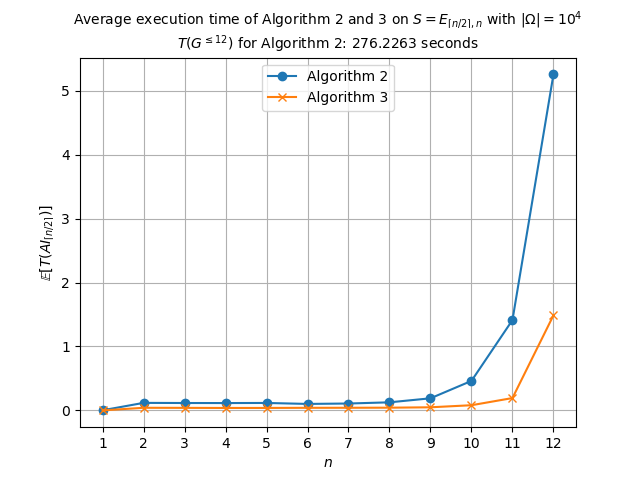
\includegraphics[width=0.8\textwidth]{images/plot_n_12_sample_10000.png}
    \caption{Average time execution per number of variables of Algorithms~\ref{alg:RMApproach} and \ref{alg:fullAlg3ForAIRestrictesSetOpt} over $10^4$ random $\WAPB{n}$ functions on the set $E_{\lceil{n/2}\rceil,n}$. 
    $T\left(G^{\leq 12}\right)$ gives the time of the pre-computation of the sequence of all Reed-Muller matrices up to $G_{12,12}$.}\label{fig:compTimePlot}
\end{figure}

The pre-computation times of $G^{\leq n_{max}}$ for Algorithm~\ref{alg:RMApproach} are given in the Table~\ref{table:preComputationTimes}. From Figure~\ref{fig:compTimePlot}, we observe that Algorithm~\ref{alg:fullAlg3ForAIRestrictesSetOpt} outperforms Algorithm~\ref{alg:RMApproach} for $n \leq 12$, even without considering the pre-computation time required for $G^{\leq n_{max}}$ and $D^{\leq n_{max}}$ in Algorithm~\ref{alg:RMApproach}. Furthermore, Algorithm~\ref{alg:RMApproach} becomes impractical for $n > 12$ due to the excessive complexity of pre-computation. In contrast, Algorithm~\ref{alg:fullAlg3ForAIRestrictesSetOpt} remains feasible for larger values of $n$. 

\begin{table}[H]
\centering
\resizebox{\textwidth}{!}{
\renewcommand{\tabcolsep}{2pt}	
\begin{tabular}{|c|c|c|c|c|c|c|c|c|c|c|c|}
%\toprule
\hline
    $G^{\leq 1}$  & $G^{\leq 2}$  &$G^{\leq 3}$  & $G^{\leq 4}$  & $G^{\leq 5}$  & $G^{\leq 6}$  & $G^{\leq 7}$  &$G^{\leq 8}$ & $G^{\leq 9}$ & $G^{\leq 10}$ & $G^{\leq 11}$  & $G^{\leq 12}$ \\
 %   \midrule
 \hline
     0.0126 & 0.0042 & 0.0017 & 0.004 & 0.0149 & 0.0470 & 0.1938 & 0.806& 3.5456& 14.9168& 65.5014 & 276.2263\\
%     \bottomrule
\hline
\end{tabular}
}
\caption{Pre-computation time (in seconds) for $G^{\leq n_{max}}$ for $n_{max}$ from $1$ to $12$.}\label{table:preComputationTimes}
\end{table}

Both implementations of the algorithms used to generate the plot in Figure~\ref{fig:compTimePlot} have been developed in \textit{Python}, with the following enhancements:
\begin{itemize}
\item The linear algebra operations in Algorithm~\ref{alg:RMApproach} are performed using the \textit{SageMath} library, while those in Algorithm~\ref{alg:fullAlg3ForAIRestrictesSetOpt} are executed using an ad-hoc custom \textit{Python} package implemented in \textit{Rust}. This setup ensures comparability between the two implementations, as the \textit{SageMath} library is highly optimized for linear algebra operations.
\item The computation of $G^{\leq n_{max}}$ for Algorithm~\ref{alg:RMApproach} is performed using the \textit{generator\_matrix} method of the \textit{SageMath} object \textit{BinaryReedMullerCodes}. While this computation could be more efficient if implemented in \textit{Rust}, the current overall implementation still faces scalability issues. Specifically, for $n \geq 16$, the algorithm becomes impractical because $G_{16,16}$ cannot be stored in a native \textit{Python} list or a \textit{SageMath} matrix object. However, if the entire algorithm were implemented in \textit{Rust}, it could potentially be feasible. Consequently, for larger values of $n$, Algorithm~\ref{alg:RMApproach} is not usable, while Algorithm~\ref{alg:fullAlg3ForAIRestrictesSetOpt} remains viable.
\end{itemize}


\section{Plots of AIk probability distributions of WPB functions and average execution times.}\label{appendix:distPlots}

\begin{figure}[H]
    \centering
    \begin{minipage}[b]{0.45\textwidth}
        \centering
        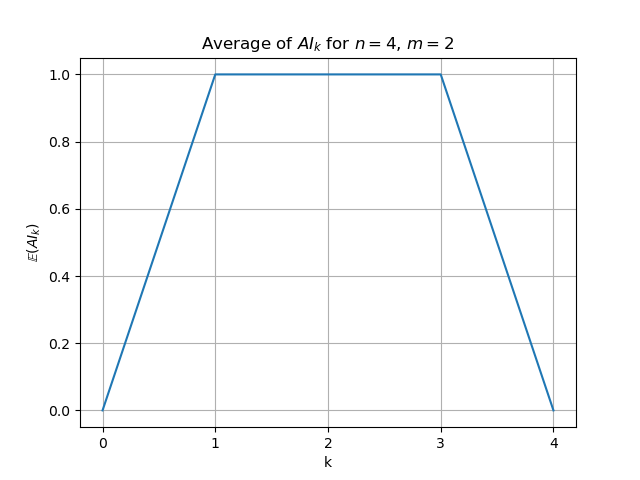
\includegraphics[width=\textwidth]{images/WPB_2_sample_size_full_dist.png}
        \caption{Mean of $\AIk{k}$ over $\WPB{2}$.}
        \label{fig:averagesFullDist}
    \end{minipage}
    \hfill
    \begin{minipage}[b]{0.5\textwidth}
        \centering
        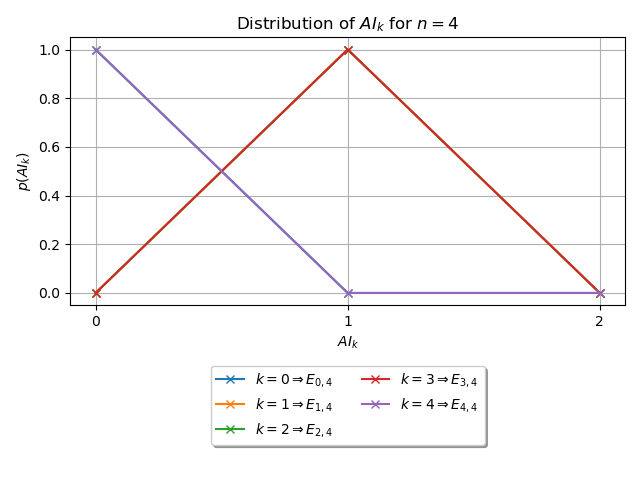
\includegraphics[width=\textwidth]{images/WPB_2_sample_size_full_dist_prob.png}
        \caption{Probability distribution of $\AIk{k}$  over $\WPB{2}$.}
        \label{fig:probFullDist}
    \end{minipage}
    \caption{Mean of $\AIk{k}$ and probability distribution of $\AIk{k}$ from Definition~\ref{def:distAIk} of $4$-variable WPB functions.}
    \label{fig:dullDist}
\end{figure}

\begin{figure}[H]
    \centering
    \begin{minipage}[b]{0.45\textwidth}
        \centering
        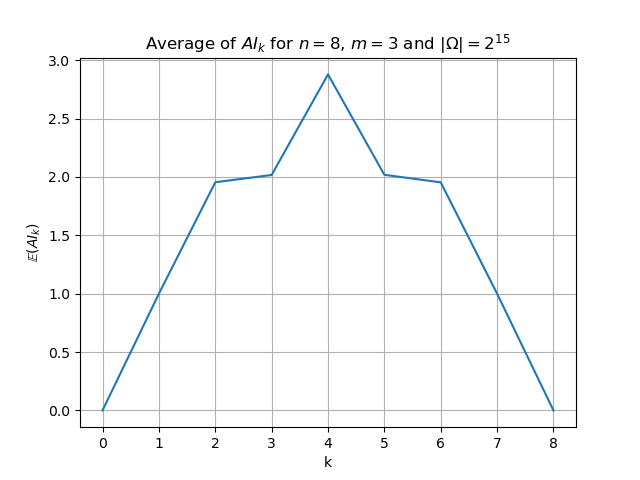
\includegraphics[width=\textwidth]{images/WPB_3_sample_size_32768_average_a.png}
        \caption{Estimated average of $\AIk{k}$ over $\WPB{3}$.}
        \label{fig:averages32768}
    \end{minipage}
    \hfill
    \begin{minipage}[b]{0.5\textwidth}
        \centering
        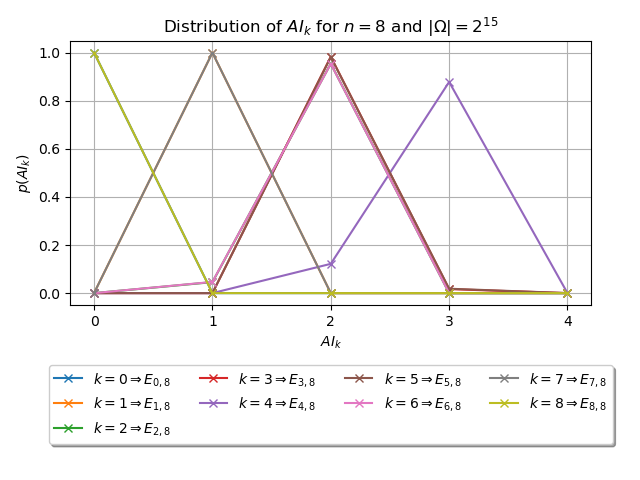
\includegraphics[width=\textwidth]{images/WPB_3_sample_size_32768_dist_prob_a.png}
        \caption{Estimated Probability distribution of $\AIk{k}$ over $\WPB{3}$.}
        \label{fig:probDist32768}
    \end{minipage}
    \caption{Estimated average of $\AIk{k}$ and probability distribution of $\AIk{k}$ over $8$-variable WPB functions, with $2^{15}$ samples.}
    \label{fig:main2}
\end{figure}

\begin{figure}[H]
    \centering
    \begin{minipage}[b]{0.45\textwidth}
        \centering
        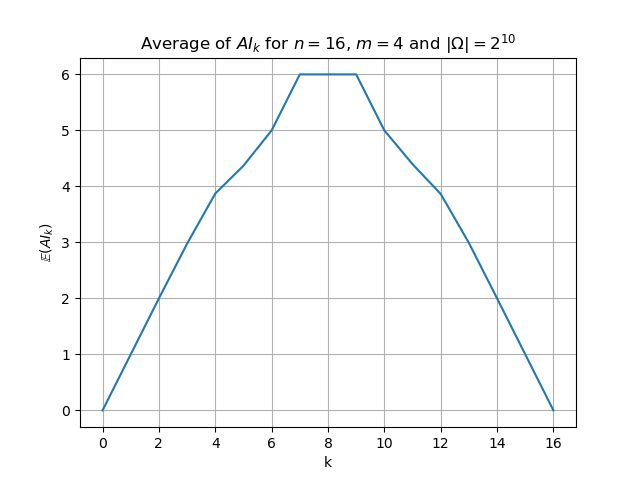
\includegraphics[width=\textwidth]{images/WPB_4_sample_size_1024_average_a.png}
        \caption{Estimated average of $\AIk{k}$ over $\WPB{4}$.}
        \label{fig:averages2014}
    \end{minipage}
    \hfill
    \begin{minipage}[b]{0.5\textwidth}
        \centering
        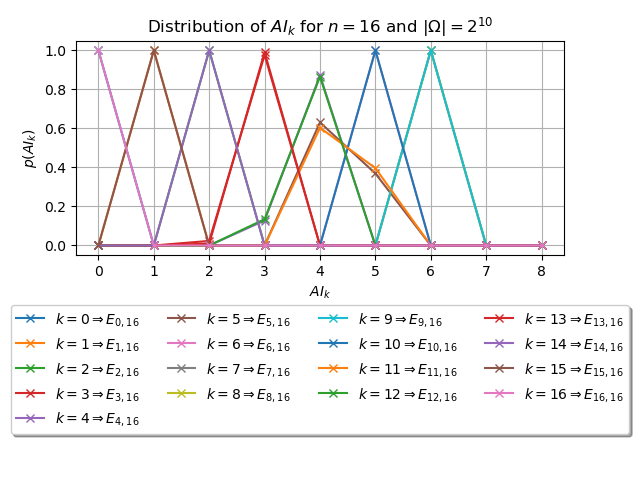
\includegraphics[width=\textwidth]{images/WPB_4_sample_size_1024_dist_prob_a.png}
        \caption{Estimated Probability distribution of $\AIk{k}$ over $\WPB{4}$.}
        \label{fig:probDist2014}
    \end{minipage}
    \caption{Estimated average of $\AIk{k}$ and probability distribution of $\AIk{k}$ over $8$-variable WPB functions, with $2^{10}$ samples.}
    \label{fig:main2014}
\end{figure}

\begin{table}
    \centering
    \caption{Averages execution times and $\AI{k}$ of $\WPB{2}$, $\WPB{3}$ and $\WPB{4}$ functions.}
    \label{table:transposed_averages}

    \begin{subtable}[t]{0.8\textwidth}
        \centering
        \caption{Average execution time and $\AIk{k}$ for $n=4$, $m=2$.}
        \label{table:averagesFullDist}
        \renewcommand{\arraystretch}{1.2}
        \renewcommand{\tabcolsep}{3pt}	
        \begin{tabular}{r|ccccc}
            \toprule
            $k$ & 0 & 1 & 2 & 3 & 4 \\
            \midrule
            $\mathbb{E}[T(AI_k)]$ & $0.53\times 10^{-4}$ & $0.0526$ & $0.0487$ & $0.0586$ & $0.6\times10^{-5}$\\
            $\mathbb{E}[AI_k]$     & $0.00$     & $1.00$     & $1.00$     & $1.00$     & $0.00$ \\
            \bottomrule
        \end{tabular}
    \end{subtable}

    \vspace{1em} % Add space between tables

    \begin{subtable}[t]{0.9\textwidth}
        \centering
        \caption{Average execution time and $\AIk{k}$ for $n=8$, $m=3$ and $\mbox{sampleSize}=2^{15}$.}
        \label{table:averages32768}
        \renewcommand{\arraystretch}{1.2}
        \resizebox{\textwidth}{!}{ % Resize to fit within page width
        \renewcommand{\tabcolsep}{3pt}	
        \begin{tabular}{r|ccccccccc}
            \toprule
            $k$ & 1 & 2 & 3 & 4 & 5 & 6 & 7\\
            \midrule
            $\mathbb{E}[T(AI_k)]$ & $0.0756$ & $0.086$ & $0.094$ & $0.090$ & $0.102$ & $0.092$ & $0.0938$ \\
            $\mathbb{E}[AI_k]$  & $1.00$     & $1.95$     & $2.02$     & $2.88$     & $2.02$     & $1.95$     & $1.00$     \\
            \bottomrule
        \end{tabular}
        }
    \end{subtable}

    \vspace{1em} % Add space between tables

    \begin{subtable}[t]{1.1\textwidth}
        \centering
        \caption{Average execution time and $\AIk{k}$ for $n=16$, $m=4$ and $\mbox{sampleSize}=2^{10}$.}
        \label{table:averages16VarsSampleSize1024}
        %\renewcommand{\arraystretch}{1.2}
        \resizebox{\textwidth}{!}{ % Resize to fit within page width
        \renewcommand{\tabcolsep}{2pt}	
        \begin{tabular}{r|cccccccccccccccccc}
            \toprule
            $k$ & 1 & 2 & 3 & 4 & 5 & 6 & 7 & 8 & 9 & 10 & 11 & 12 & 13 & 14 & 15\\
            \midrule
            $\mathbb{E}[T(AI_k)]$ & $0.334$ & $0.342$ & $0.41$ & $4.01$ & $91.81$ & $636.37$ & $2838.92$ & $6384.38$ & $3111.12$ & $732.50$ & $118.96$ & $5.23$ & $0.43$ & $0.35$ & $0.35$\\
            $\mathbb{E}[AI_k]$ & $1.00$     & $2.00$     & $2.99$     & $3.89$     & $4.37$     & $5.00$     & $6.00$     & $6.00$     & $6.00$     & $5.00$     & $4.40$     & $3.87$     & $2.99$     & $2.00$     & $1.00$\\
            \bottomrule
        \end{tabular}
        }
    \end{subtable}
\end{table}

\end{document}
